\documentclass[]{foi} % zakomentirati za pisanje rada na engleskom jeziku
% \documentclass[english]{foi} % odkomentirati za pisanje rada na engleskom jeziku
\usepackage[utf8]{inputenc}
\usepackage{lipsum}

\vrstaRada{\seminar}
% \zavrsni ili \diplomski ili \seminar ili \projekt

\title{Naslov rada -- LaTeX Predložak}
\predmet{\predmetTBP}
% ostaviti prazno ako \vrstaRada nije \projekt ili \seminar
% \predmetBP ili \predmetDP ili \predmetTBP ili \predmetVAS

\author{Barica} % ime i prezime studenta/studentice
\spolStudenta{\zensko} % \zensko ili \musko

\mentor{Bogdan Okreša Đurić} % ime i prezime mentora
\spolMentora{\musko} % \zensko ili \musko
\titulaProfesora{dr. sc.}
% HR: dr. sc.  / doc. dr. sc. / izv. prof. dr. sc. / prof. dr. sc. 
% EN: -prazno- / Asst. Prof.  / Assoc. Prof.       / Full Prof.

\godina{2022}
\mjesec{rujan} % mjesec obrane rada ili projekta

\indeks{35918/07–R} % broj indeksa ili JMBAG

\smjer{Informacijski i poslovni sustavi}
% (ili:
%     Informacijski sustavi, 
%     Poslovni sustavi, 
%     Ekonomika poduzetništva, 
%     Primjena informacijske tehnologije u poslovanju, 
%     Informacijsko i programsko inženjerstvo, 
%     Baze podataka i baze znanja, 
%     Organizacija poslovnih sustava, 
%     Informatika u obrazovanju
% )


\sazetak{Opsega od 100 do 300 riječi. Sažetak upućuje na temu rada, ukratko se iznosi čime se rad bavi, teorijsko-metodološka polazišta, glavne teze i smjer rada te zaključci.}

\kljucneRijeci{riječ; riječ; ...riječ; Obuhvaća $7\pm2$ ključna pojma koji su glavni predmet rasprave u radu.}



\begin{document}

\maketitle

\tableofcontents

\makeatletter \def\@dotsep{4.5} \makeatother
\pagestyle{plain}



\chapter{Uvod}

Tema ovog rada je izrada online igrice pomoću objektno-orijentirane baze podataka (OOBP). Kako je sve veća potreba za izgradnjom sustava sa što većom sličnošću baze podataka i aplikacijske domene dovelo je do objektno-orijentiranog pristupa izgradnje baze podataka. OOBP je baza podataka u koju pohranjujemo podatke u obliku objekata za razliku od klasičnih baza podataka gdje je podatak pohranjen u obliku tablice (relacije). Objektno-orijentirane aplikacije manipuliraju objektima te pri ponovnom pokretanju aplikacije dolazi do brisanja podataka objekata, stoga moramo imati nekakav mehanizam upravljana spremanja podataka. Za izgradnju online igrice uzeta je poznata igra Križić kružić te pomoću ZODB (Zope Object Data Base), koji omogućava pohranu objekata u programskom jeziku Python, kreirana aplikacija Križić kružić koja se može igrati u više igrača preko mreže te koja spremanja podataka za kasniju upotrebu. 
.



\chapter{Korišteni alati}

ZODB pohranjuje Python proširenjem (engl. Extend) objekte koristeći ugrađene Persistent klase. ZODB baza podataka ima jedan korijenski objekt tipa rječnik, koji je jedini objekt kojem baza podataka izravno pristupa. Svi ostali objekti pohranjeni u bazi podataka dostupni su preko korijenskog objekta. Objekti na koje upućuje objekt pohranjen u bazi podataka također se automatski pohranjuju u bazu podataka. Budući da je ZODB objektna baza podataka nema zasebnog jezika za operacije baze podataka, vrlo mali utjecaj na vaš kod kako bi objekti bili postojani, nema mapera baze podataka koji djelomično skriva bazu podataka. Korištenje objektno-relacijskog preslikavanja nije kao korištenje objektne baze podataka. Gotovo da nema spojeva između koda i baze podataka. Odnosima između objekata rukuje se vrlo prirodno, podržavajući složene objektne grafikone bez spojeva (engl. joins). [1]

Zope Enterprise Objects (ZEO) implementacija je ZODB pohrane koja omogućuje višestrukim klijentskim procesima da pristupe spremljenim objektima na jednom ZEO poslužitelju. To omogućuje transparentno skaliranje. Kada koristite ZEO, pohrana niže razine, obično pohrana datoteka, otvara se u procesu ZEO poslužitelja. Klijentski programi povezuju se s ovim procesom koristeći ZEO ClientStorage. ZEO pruža dosljedan prikaz baze podataka svim klijentima. ZEO klijent i poslužitelj komuniciraju korištenjem prilagođenog protokola slojevitog na vrhu TCP-a.[3]

ZODB preglednik vam omogućuje pregled postojanih objekata pohranjenih u ZODB-u, pregled njihovih atributa i povijesnih promjena koje su na njima napravljene. [4]


\chapter{Korišteni alati}

Dijagram klasa prikazan na slici [1] prikazuje model baze podataka koji se sastoji od objekata Korisnik, Igra i Ploca koji su povezani agregacijskom vezom. Klasa Aplikacija je glavna klasa igrice Križić kružić te se on instancira na svakom pokretanju aplikacije. Sadrži varijable i funkcije za pokretanje, igranje i komunikaciju s bazom podataka.

\begin{figure}[]
    \centering
    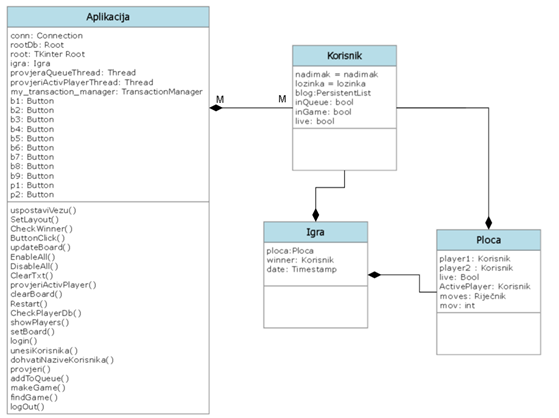
\includegraphics[width=0.9\textwidth]{slike/klas.png}
    \caption{Klas dijagram \cite{Vlastita izrada}}
    \label{fig:podjela}
\end{figure}

Kreirana baza podataka u sebi sadrži korijenski objekt root tipa rječnik u kojega se spremaju podaci. U tablici [1] je prikazana hijerarhijska struktura root objekta gdje vidimo ostale objekte sadržane u root objektu, ključ objekta i tip.


\begin{figure}[]
    \centering
    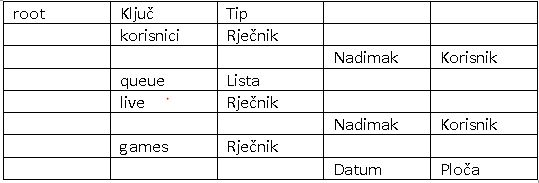
\includegraphics[width=0.9\textwidth]{slike/tablica_root.jpg}
    \caption{Klas dijagram \cite{Vlastita izrada}}
    \label{fig:podjela}
\end{figure}


\chapter{Primjer korištenjai}


U sljedećem poglavlju opisano je pokretanje servera sa bazom podataka i pokretanje izvođenje aplikacije. Također za potrebe prikaza sadržaja baze van aplikacije korištena je ZODB browser plugin.




\section{Pokretanje servera }


Kao bi naša baza podataka bila dostupna prvo ju pokrećemo iz terminala naredbom sa slike [2] i naredbom sa slike [3] pokrećemo zodb browser preglednik za ZODB.



\begin{figure}[]
    \centering
    
\includegraphics[width=0.9\textwidth]{slike/runzeo_command.png}
    \caption{Runzeo naredba \cite{Vlastita izrada}}
    \label{fig:podjela}
\end{figure}


\begin{figure}[]
    \centering
    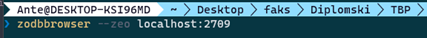
\includegraphics[width=0.9\textwidth]{slike/browser_command.png}
    \caption{ZODB browser naredba \cite{Vlastita izrada}}
    \label{fig:podjela}
\end{figure}


\section{Pokretanje aplikacij i prijava}

Aplikaciju pokrećemo kroz naredbenu konzolu kao python skriptu. Nakon pokretanja aplikacije prikazati će se iskočni prozor, slika [4], s mogućnosti unosa nadimka igrača, u slučaju da igrač s nadimkom ne postoji kreira se novi igrač i igra može započet.


\begin{figure}[]
    \centering
    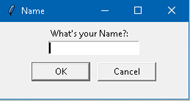
\includegraphics[width=0.9\textwidth]{slike/login.png}
    \caption{Login prozor \cite{Vlastita izrada}}
    \label{fig:podjela}
\end{figure}


\section{Igranje}

Kada se korisnik spoji na aplikaciju unosom nadimka prikazuje se prozor s aplikacijom i gumbima koje može pritiskati nakon što se pronađe protivnik. Igrač može samostalno biti logiran ili ubaciti sebe u red čekanja za pronalazak protivnika. Na slici [5] vidimo dvije instance aplikacije pokrenute i svaka pokazuje listu aktivnih igrača s desne strane koja se ažurira svakih par minuta.

Pritiskom na gumb Play igrača se dodaje u red čekanja za pronalazak protivničkog igrače te će se gumbi tj. polja za poteze odblokirati kada se pronađe protivnički igrač prikazano na slici [5]. Slika [6] prikazuje dva igrača (a i b) koja su uparena iz reda čekanja te je pokrenuta nova igra. Na potezu je igrač „a“ i kao prvi igrač ima oznaka „x“

\begin{figure}[]
    \centering
    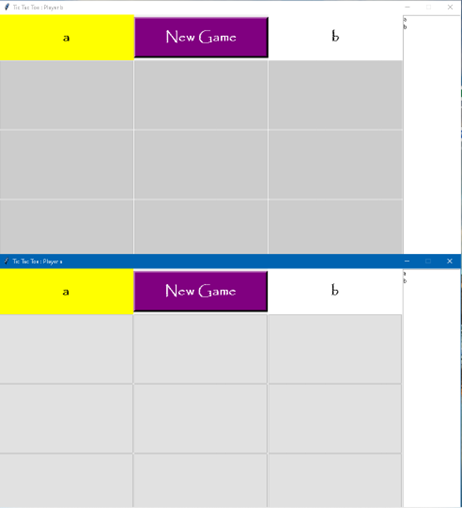
\includegraphics[width=0.9\textwidth]{slike/igranje_2.png}
    \caption{Započeta igra s dva igrača \cite{Vlastita izrada}}
    \label{fig:podjela}
\end{figure}


.
Na pritisak korisnik na prazno polje unosi se oznaka sa simbolom korisnika koji je bio na redu te se žuta boja igrača mijenja na protivničkog igraća. Svaku sekundu u pozadini se ispituje dali je došlo do zapisa poteza u bazi podataka te se potez sa slike [7] igraća „a“ prikazuje na protivničkoj ploče i polja se blokiraju za daljnji unos dok protivnički „b“ igrač ne napravi potez..

\begin{figure}[]
    \centering
    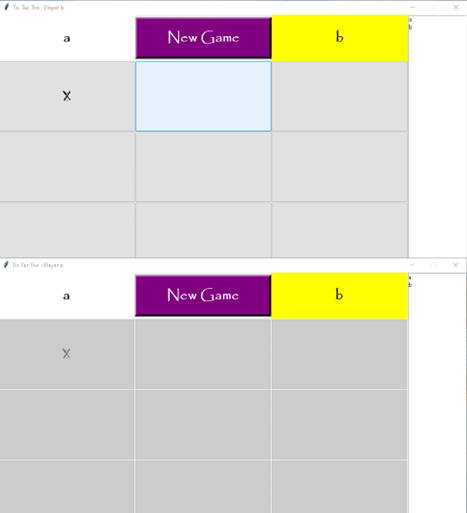
\includegraphics[width=0.9\textwidth]{slike/igranje_3.png}
    \caption{Prvi potezi igrača \cite{Vlastita izrada}}
    \label{fig:podjela}
\end{figure}


Na slici [8] je prikazana završena runda između igraća „a“ i „b“, nakon što je jedan od njih u ovom slučaju b igrač postavio tri uzastopna simbola „X“ osvježio se zadnji prikaz svih poteza igra se zaustavila i prikazao se iskočni prozor s porukom o pobjedi igraća „b“ za obje pokrenute aplikacije. Pritiskom na gumb „Ok“ aplikacija obriše poteze igraća te se igraći ponovno mogu dodijeliti u red čekanja na protivnika.



\begin{figure}[]
    \centering
    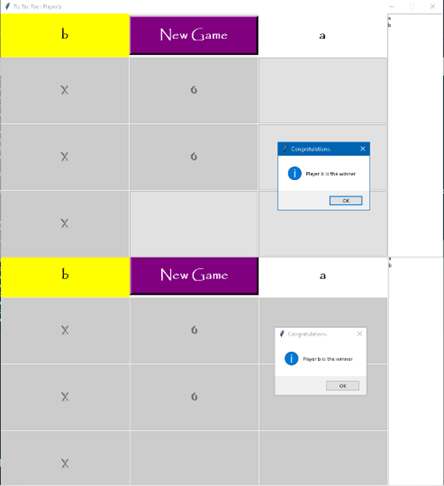
\includegraphics[width=0.9\textwidth]{slike/igranje_4.png}
    \caption{Kraj igre \cite{Vlastita izrada}}
    \label{fig:podjela}
\end{figure}




\section{Implementacija}


U sljedećih par poglavlja biti će opisane pojedine implementacije funkcionalnosti aplikacije. 


\section{Model}


Klase sa slike [9] prikazuju objekte Igru, Plocu, Korisnika i aplikaciju koji se koriste u aplikaciji. Aplikacija je glavna klasa aplikacije koja upravlja objektima i podacima za igranje igre, self.provjeraQueueThread i self.provjeraActivePlayerThread su dvije niti koje se vrte u pozadini aplikacije sve dok se aplikacije ne zaustavi. Klase Igra, Ploca i korisnik se koriste u aplikaciji za prijeno podatak ali i ZODB pomoću njih kreira pogleda (view) na bazu podataka koje vidi aplikacija prilikom komunikacije s bazom. 


\begin{figure}[]
    \centering
    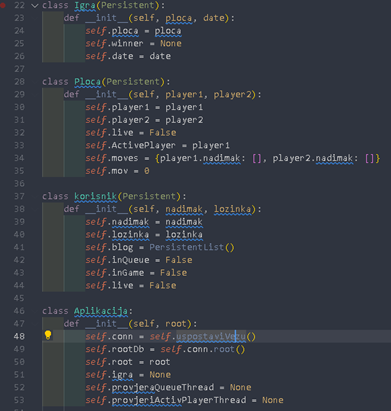
\includegraphics[width=0.9\textwidth]{slike/impl_1.png}
    \caption{Klase aplikacije \cite{Vlastita izrada}}
    \label{fig:podjela}
\end{figure}


\section{Konekcija na server}

Kako se u aplikaciji koristi više niti na kreiranju konekcije s bazom moramo imati tzv. Transactionmanagera koji se brine o našim transakcijama. Kreiramo ClienStorage na prije pokrenutom serveru  [10] te instancu baze te otvaramo konekciju prema bazi s TransactionMaangerom i to je naša pristupna točka.

\begin{figure}[]
    \centering
    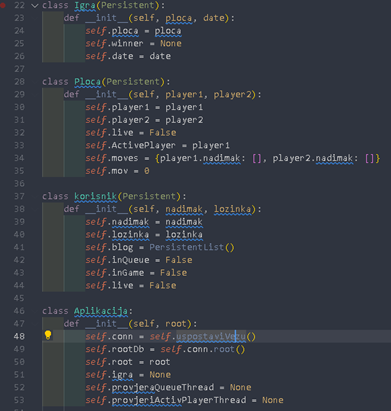
\includegraphics[width=0.9\textwidth]{slike/impl_1.png}
    \caption{Metoda uspostaviVezu \cite{Vlastita izrada}}
    \label{fig:podjela}
\end{figure}



\section{Traženje protivnika – queue}

Pritiskom na gumb Play postavlja sebe na red čekanja za odabir protivnika. Slika [11] prikazuje dio koda kod koje ga se korisnik unosi u red čekanja tzv. queue i postavljaju se zastavice inQueue te se kreira transakcija i pohranjuje u bazu podataka s metodom commit(), ako je transakcija uspjela započinje izvođenje nove niti provjeraQueueThread s metodom self.provjeraQueue



\begin{figure}[]
    \centering
    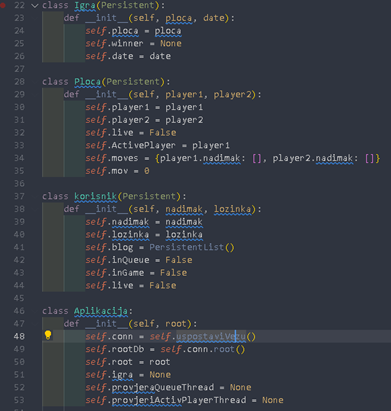
\includegraphics[width=0.9\textwidth]{slike/impl_1.png}
    \caption{Metoda addToQueue \cite{Vlastita izrada}}
    \label{fig:podjela}
\end{figure}


Metode provjeraQueue i dohvatuQueueKorisnika se izvode u novokreiranoj niti, slike [12], odgovorne su za dohvaćanje novog korisnika iz reda čekanja sve dok se takav korisnik ne postavi u red čekanja.  provjeraQueue poziva metodu dohvatiQueueKorisnika koja joj vraća pronađenog korisnika  u slučaju da je našla korisnika i trenutni korisnik nije više u queu (zastavica kor.inQueue) kreira se nova igra inače provjerava se dali je trenutni korisnik u igri (zastavica kor.inGame) te se pretražuje baza podataka s igrama, metoda findGame().


\begin{figure}[]
    \centering
    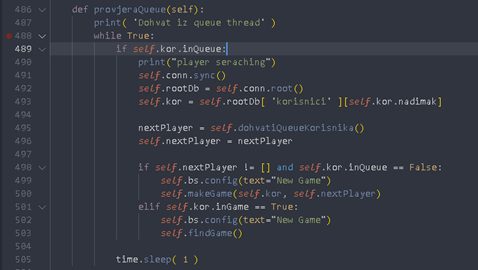
\includegraphics[width=0.9\textwidth]{slike/impl_4.png}
    \caption{Metoda provjeraQueue \cite{Vlastita izrada}}
    \label{fig:podjela}
\end{figure}


Metoda dohvatiQueueKorisnika, slika [13], dohvaća prvog korisnika u queue te ako je taj korisnik različit od trenutnog briše ga iz queue i briše trenutnog korisnika iz queue, postavlja atribute inQueu za oba korisnike na True, zapisuje promjene u bazu i pronađenog korisnika vraća kao povratnu vrijednost.


\begin{figure}[]
    \centering
    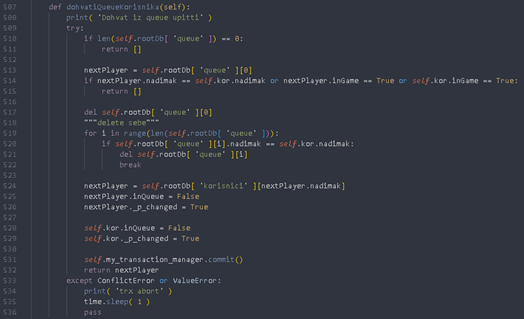
\includegraphics[width=0.9\textwidth]{slike/impl_5.png}
    \caption{Metoda dohvatiQueueKorisnika \cite{Vlastita izrada}}
    \label{fig:podjela}
\end{figure}


\section{Kreiranje igre}

Kod kreiranja nov igre, metoda makeGame prihvaća argumente player1 i player2 te instanciranje objekt Ploca i Igra. Igri se dodjeljuju poslani player1 i player2 te se igri dodaje instancirana ploca. Igracima se postavlja parametar inGame na vrijednsot True kako bi protivnički igrač mogao pronać igru, slika [16 ], a ne kreirati novu.


\begin{figure}[]
    \centering
    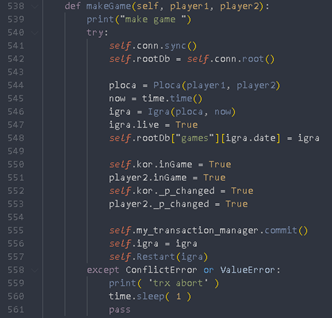
\includegraphics[width=0.9\textwidth]{slike/impl_6.png}
    \caption{Metoda makeGame \cite{Vlastita izrada}}
    \label{fig:podjela}
\end{figure}



Igrač koji je pronađen u queue od strane drugog igrača koji je kreirao igru, ne kreira novu igru već pronalazi već kreiranu igru preko atributa date objekta igra. Metoda findGame, slika [17], pronalazi prvu igru koja se izvodi iz baze s igračem koji je dodijeljen toj igri.



\begin{figure}[]
    \centering
    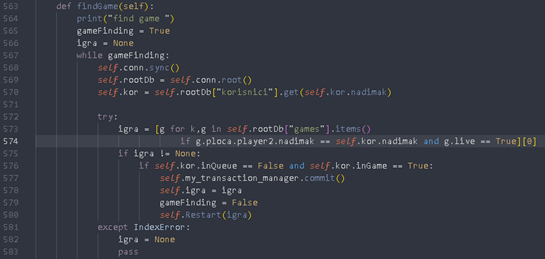
\includegraphics[width=0.9\textwidth]{slike/impl_7.png}
    \caption{Metoda findGame \cite{Vlastita izrada}}
    \label{fig:podjela}
\end{figure}

\section{Potez igrača}


Svakom polju na ploči dodijeljen je event pritiska tipke miša. Prilikom pritiska tipke miša poziva se metoda ButtonClick koja ažurira root objekt, provjerava koji je trenutni aktivni igrač u objektu ploca te ako je trenutni korisnik aplikacije aktivni igrač dopušta mu postavljane simbola na pritisnuto polje. Mijenja se aktivni igrač u suigrača i promjene se pohranjuju u bazu. Slika [18]

\begin{figure}[]
    \centering
    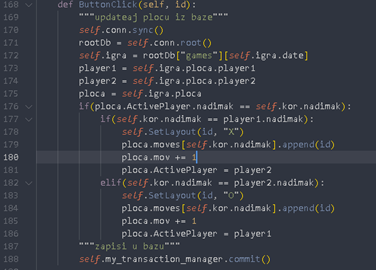
\includegraphics[width=0.9\textwidth]{slike/impl_8.png}
    \caption{Metoda ButtonClick \cite{Vlastita izrada}}
    \label{fig:podjela}
\end{figure}


OPIS

\begin{figure}[]
    \centering
    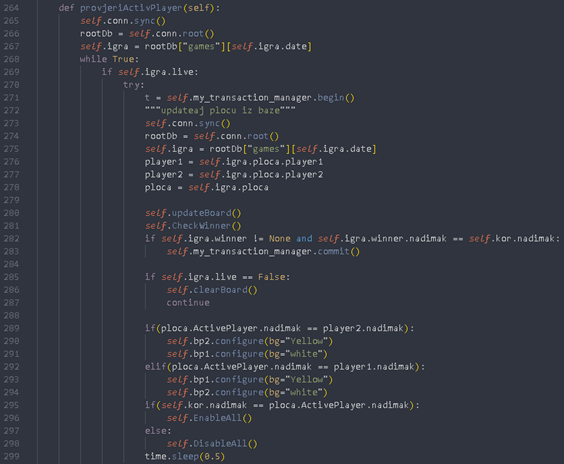
\includegraphics[width=0.9\textwidth]{slike/impl_9.png}
    \caption{Metoda ButtonClick \cite{Vlastita izrada}}
    \label{fig:podjela}
\end{figure}




\section{Potez igrača}

Svaka ploča ima atribut s vrijednostima poteza za svakog igrača spremljenog u obliku rječnika. Ako se u nekoj listi korisnika nađe uzastopnih tri poteza slika [19] taj korisnik je pobjednik.  Na kraju postavljamo atribute winner, inGame i live te prikazujemo poruku o pobjedniku slika [20 ].

\begin{figure}[]
    \centering
    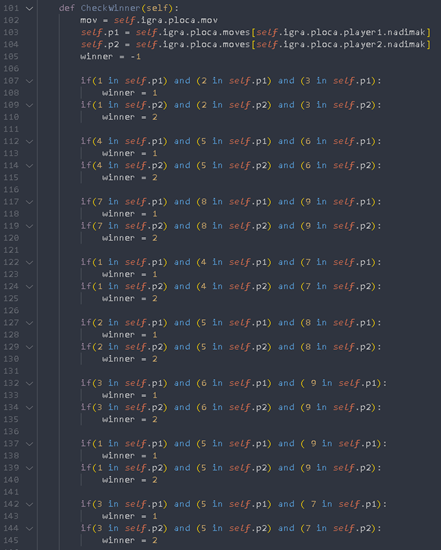
\includegraphics[width=0.9\textwidth]{slike/impl_10.png}
    \caption{Metoda ButtonClick a \cite{Vlastita izrada}}
    \label{fig:podjela}
\end{figure}


\begin{figure}[]
    \centering
    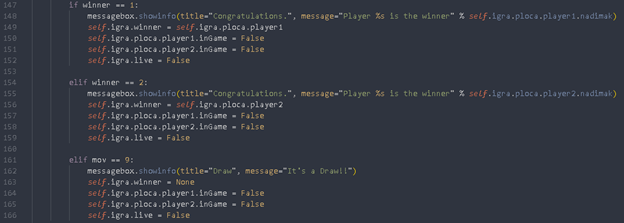
\includegraphics[width=0.9\textwidth]{slike/impl_11.png}
    \caption{Metoda ButtonClick b \cite{Vlastita izrada}}
    \label{fig:podjela}
\end{figure}


\section{Odjava}

Prilikom odjave korisnika postavljaju se atributi live, inQueu, inGame na False kaok bi osigurali da ne dođe do rešenja aplikacije prilikom ponovnog pokretanja i brišemo objekte iz baze spremljen u live i queue rječnike. Slika [21]
\begin{figure}[]
    \centering
    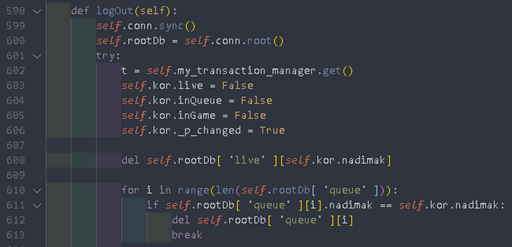
\includegraphics[width=0.9\textwidth]{slike/impl_12.png}
    \caption{Metoda logOut \cite{Vlastita izrada}}
    \label{fig:podjela}
\end{figure}

Prilikom zatvaranja aplikacije postavljamo zastavice jos, next na fals kako bi prekinuli izvođenje petlji u nitima te uništava se korijen korisničkog sučelja i poziv metode logOut. Slika [22]

\begin{figure}[]
    \centering
    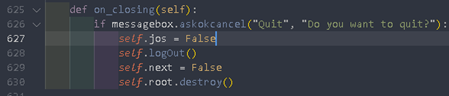
\includegraphics[width=0.9\textwidth]{slike/impl_13.png}
    \caption{Metoda logOut \cite{Vlastita izrada}}
    \label{fig:podjela}
\end{figure}



\chapter{Zaključak}

\chapter{Bibliografija}


\end{document}
